\documentclass[conference]{IEEEtran}
%\IEEEoverridecommandlockouts
% The preceding line is only needed to identify funding in the first footnote. If that is unneeded, please comment it out.
\usepackage{cite}
\usepackage{amsmath,amssymb,amsfonts}
\usepackage{algorithmic}
\usepackage{graphicx}
\usepackage{textcomp}
\usepackage{xcolor}
\def\BibTeX{{\rm B\kern-.05em{\sc i\kern-.025em b}\kern-.08em
    T\kern-.1667em\lower.7ex\hbox{E}\kern-.125emX}}

\usepackage{siunitx}
\usepackage{listings}
% Copyright 2017 Sergei Tikhomirov, MIT License
% https://github.com/s-tikhomirov/solidity-latex-highlighting/

\usepackage{listings, xcolor}

\definecolor{verylightgray}{rgb}{.97,.97,.97}

\lstdefinelanguage{Solidity}{
	keywords=[1]{anonymous, assembly, assert, balance, break, call, callcode, case, catch, class, constant, continue, constructor, contract, debugger, default, delegatecall, delete, do, else, emit, event, experimental, export, external, false, finally, for, function, gas, if, implements, import, in, indexed, instanceof, interface, internal, is, length, library, log0, log1, log2, log3, log4, memory, modifier, new, payable, pragma, private, protected, public, pure, push, require, return, returns, revert, selfdestruct, send, solidity, storage, struct, suicide, super, switch, then, this, throw, transfer, true, try, typeof, using, value, view, while, with, addmod, ecrecover, keccak256, mulmod, ripemd160, sha256, sha3}, % generic keywords including crypto operations
	keywordstyle=[1]\color{blue}\bfseries,
	keywords=[2]{address, bool, byte, bytes, bytes1, bytes2, bytes3, bytes4, bytes5, bytes6, bytes7, bytes8, bytes9, bytes10, bytes11, bytes12, bytes13, bytes14, bytes15, bytes16, bytes17, bytes18, bytes19, bytes20, bytes21, bytes22, bytes23, bytes24, bytes25, bytes26, bytes27, bytes28, bytes29, bytes30, bytes31, bytes32, enum, int, int8, int16, int24, int32, int40, int48, int56, int64, int72, int80, int88, int96, int104, int112, int120, int128, int136, int144, int152, int160, int168, int176, int184, int192, int200, int208, int216, int224, int232, int240, int248, int256, mapping, string, uint, uint8, uint16, uint24, uint32, uint40, uint48, uint56, uint64, uint72, uint80, uint88, uint96, uint104, uint112, uint120, uint128, uint136, uint144, uint152, uint160, uint168, uint176, uint184, uint192, uint200, uint208, uint216, uint224, uint232, uint240, uint248, uint256, var, void, ether, finney, szabo, wei, days, hours, minutes, seconds, weeks, years},	% types; money and time units
	keywordstyle=[2]\color{teal}\bfseries,
	keywords=[3]{block, blockhash, coinbase, difficulty, gaslimit, number, timestamp, msg, data, gas, sender, sig, value, now, tx, gasprice, origin},	% environment variables
	keywordstyle=[3]\color{violet}\bfseries,
	identifierstyle=\color{black},
	sensitive=true,
	comment=[l]{//},
	morecomment=[s]{/*}{*/},
	commentstyle=\color{gray}\ttfamily,
	stringstyle=\color{red}\ttfamily,
	morestring=[b]',
	morestring=[b]"
}

\lstset{
	language=Solidity,
	backgroundcolor=\color{verylightgray},
	extendedchars=true,
	basicstyle=\footnotesize\ttfamily,
	showstringspaces=false,
	showspaces=false,
	numbers=left,
	numberstyle=\footnotesize,
	numbersep=9pt,
	tabsize=2,
	breaklines=true,
	showtabs=false,
	captionpos=b
}


\makeatletter
\def\ps@IEEEtitlepagestyle{%
  \def\@oddfoot{\mycopyrightnotice}%
  \def\@evenfoot{}%
}
\def\mycopyrightnotice{%
  {\footnotesize \textnormal{979-8-3503-4647-3/23/\$31.00 ©2023 IEEE}\hfill}
  \gdef\mycopyrightnotice{}
}

\renewcommand\IEEEkeywordsname{Keywords} % Change "Index Terms" to "Keywords"

\begin{document}

\title{Token Composition: A Graph-Based Exploration of Ethereum Event
  Logs
%\thanks{Identify applicable funding agency here. If none, delete this.}
}

\author{
\IEEEauthorblockN{Martin Harrigan}
\IEEEauthorblockA{\textit{Dept.\ of Computing, Carlow Campus}\\
\textit{South East Technological University}\\
Rep.\ of Ireland\\
martin.harrigan@setu.ie}
\and
\IEEEauthorblockN{Thomas Lloyd}
\IEEEauthorblockA{\textit{Dept.\ of Computing, Carlow Campus}\\
\textit{South East Technological University}\\
Rep.\ of Ireland\\
tomlloyd1992@gmail.com}
\and
\IEEEauthorblockN{Daire O'Broin}
\IEEEauthorblockA{\textit{Dept.\ of Computing, Carlow Campus} \\
\textit{South East Technological University}\\
Rep.\ of Ireland\\
daire.obroin@setu.ie}
}

\maketitle

\begin{abstract}
  Tokens are proliferating across blockchains in terms of number, market
capitalisation and utilty.  Some tokens are tokenised versions of
existing tokens --- known variously as wrapped tokens, fractional
tokens, or shares.  The repeated application of this process creates
matryoshkian tokens of arbitrary depth.  We perform an empirical
analysis of token composition on the Ethereum blockchain.  We
introduce a graph that represents the tokenisation of tokens by other
tokens, and we show that this graph contains non-trivial topological
structure.  We relate properties of the graph, e.g., connected
components and cyclic structure, to the tokenisation process.  For
example, we identify the longest directed path and its corresponding
sequence of tokens, and we visualise the connected components relating
to a stablecoin and an NFT protocol.  Our goal is to explore and
visualise what has been wrought, rather than add yet another brick to
the edifice of tokens.



  \begin{IEEEkeywords}
    blockchain, tokens, tokenisation, decentralised finance
  \end{IEEEkeywords}
\end{abstract}

\section{Introduction}\label{sec:introduction}

We are witnessing a Cambrian explosion of tokens on blockchains:
Ethereum alone has hundreds of thousands of ERC-20 tokens.  Many
tokens are simple, in the sense that they are not composed of other
tokens.  But, some are.  For example, a liquidity pool token
represents a share of a collection of other tokens.  DEX
Screener~\cite{dex-screener-xx}, a popular liquidity pool tracker,
lists over one hundred thousand liquidity pool tokens.  Furthermore,
tokens are being composed in ever more creative ways:
\texttt{PT-weETH-25APR2024}~(\texttt{0xb18c87}) is a token issued by
Pendle Finance~\cite{nguyen-vuong-22} on the Arbitrum blockchain that
transitively depends on many other tokens.  At the time of writing,
this token has a market capitalisation of over one billion US dollars.
It is critical from the perspectives of technical and financial risk
to examine the composition of tokens.  If an investor purchases
\texttt{PT-weETH-25APR2024}, what tokens does the investment depend
upon?  In this paper, we present a novel method of examining token
composition at both the macro- and micro-level and we apply it to the
Ethereum blockchain.

% Antoher good example: Staked Curve.fi renBTC/wBTC Convex Deposit on
% Abra (\texttt{stkcvxcrvRenWBTC-abra})

Our method extracts \textit{meta-events} from EVM logs.  Low-level
events are emitted by contracts.  Meta-events are identified by
heuristics.  A single meta-event can be derived from multiple events.
For example, ERC-20 tokens (should) emit a \texttt{Transfer} event
whenever a token is transferred~\cite{vogelsteller-buterin-15}.  A
meta-event could signify a token being tokenised by another token,
i.e., a deposit of an underlying token with a contract and the minting
of a new share, or the burning of a share and the withdrawal of an
underlying token from a contract.  This meta-event, which we will call
a \textit{tokenising meta-event}, can be identified from multiple
\texttt{Transfer} events within a single transaction.  The tokenising
meta-events can be represented as a \textit{token graph}: each vertex
represents a token and each directed edge represents the token
corresponding to the source vertex being tokenised by the token
corresponding to the target vertex.  We apply various forms of graph
analysis to the token graph and we visualise the structure of token
compositions.

This paper is organised as follows.  In Sect.~\ref{sec:related-work}
we review related work.  In Sect.~\ref{sec:token-composition} we
introduce token composition, the token graph, and our data sources.
We present our analysis in Sect.~\ref{sec:analysis}.  Finally, we
conclude in Sect.~\ref{sec:conclusion}.


\section{Related Work}\label{sec:related-work}

We categorise related work into four areas: empirical analysis of
smart contract composition and code reuse, the automatic detection of
tokens, graph analysis of blockchains and token systems, and wrapped
tokens.

Software composition is a hard problem~\cite{garlan-et-al-94}.  Smart
contracts on blockchains sidestep the low-level problems of
interoperability by using a shared execution environment (i.e., a
virtual machine) and de facto standards (e.g., ERCs), and the
high-level problems of architectural mismatch by taking a bottom-up
approach to composition.  He et al.~\cite{he-et-al-20} perform a
large-scale analysis of \num{10} million Ethereum smart contracts
deployed between July 2015 and December 2018.  They show that less
than \num{1}\% of the \num{10} million smart contracts are distinct,
and more than \num{63}\% of those are similar to at least one other
smart contract.  The results have been
replicated.~(\hspace{1sp}\cite{kondo-et-al-20,chen-et-al-21,khan-et-al-22})

Fr\"owis et al.~\cite{frowis-et-al-19} use symbolic execution to
automatically detect smart contracts on the Ethereum blockchain that
implement token functionality.  Di Angelo and
Salzer~\cite{di-angelo-salzer-21} reconstruct contract interfaces and
events from EVM bytecode.  Using primarily transaction data they
identify token contracts that comply with ERC standards and token
contracts that do not.  Oliveira et al.~\cite{oliveira-et-al-18}
propose a taxonomy for classifying tokens and they propose a decision
tree to guide the token design process.

Kitzler et al.~\cite{kitzler-et-al-21} select and analyse a subset of
DeFi activity on the Ethereum blockchain.  They construct and
topologically analyse two graphs: the \textit{contract account graph}
where the vertices are contract accounts and the edges are
transactions between those accounts, and the \textit{protocol graph}
where the vertices are protocols and the edges are transactions
between those protocols.  They show that community finding algorithms
identify communities in the contract account graph, but the
communities do not correspond to protocols.  There are several network
analyses of ERC-20 tokens on the Ethereum blockchain that quantify
their age, economic value, activity volume,
etc.~(\hspace{1sp}\cite{somin-et-al-18,victor-luders-19})

Caldarelli~\cite{caldarelli-21} discusses wrapped tokens and their
ability to represent real-world assets (tokenisation) and to bridge
tokens across blockchains (cross-blockchain interoperability).  The
WBTC whitepaper~\cite{kyber-et-al-xx} describes a general framework
for tokenising assets on a blockchain.  Santoro et
al.~\cite{santoro-et-al-22} propose a standard interface for vaults
for ERC-20 tokens.  The vaults can store a single \textit{asset} or
underlying token.  Users can \textit{deposit} or \textit{withdraw} the
asset.  In return, they receive \textit{shares} in the form of another
ERC-20 token.  Lloyd et al.~\cite{lloyd-et-al-23} analysed the
emergent outcomes of veTokens where a token is locked in exchange for
voting rights.

We use common terminology from graph theory through-out the paper.
Please refer to \cite{diestel-17} or a similar reference for
definitions.


\section{Token Composition}\label{sec:token-composition}

Tokens are central to blockchain-based protocols and
applications~\cite{voshmgir-20}.  Token composition is a technique
where one or more tokens can be combined to create new tokens.  The
entitlements of the input tokens are appropriated by the new token.
We extract data from EVM logs (Sec.~\ref{sec:token-comp-evm-logs}) and
use it to construct a token graph
(Sec.~\ref{sec:token-comp-token-graph}), a representation of the
tokenisation process.  In Sec.~\ref{sec:analysis} we will analyse the
graph and relate it to the tokenisation process.

\subsection{EVM Logs, Events and Meta-Events}\label{sec:token-comp-evm-logs}

EVM logs record specific occurrences or outputs generated during the
execution of contract code.  They enable off-chain applications to
react to on-chain events.  A popular event is the \texttt{Transfer}
event emitted by ERC~20 tokens~\cite{vogelsteller-buterin-15}:

\begin{lstlisting}[language=Solidity,numbers=none,
    caption={The ERC~20 \texttt{Transfer} event specifies three
      parameters: \texttt{from}, \texttt{to}, and \texttt{value}.}]
  event Transfer(address indexed from,
                 address indexed to,
                 uint256 value);
\end{lstlisting}

The event has two special cases.  If the \texttt{from} address is the
zero address (\texttt{0x0}) then the contract mints new tokens.  If
the \texttt{to} address is the zero address then it burns existing
tokens.

A single transaction can emit multiple events.  We define a
\textit{meta-event} to be a sequence of events that match some pattern
and are emitted by a single transaction.  We define a
\textit{tokenising meta-event} to be a meta-event where the pattern is
two \texttt{Transfer} events: one must indicate a transfer of tokens
to the contract and another must indicate a new token being minted
(\textit{deposit \& mint}), or one must indicate a token being burned
and another must indicate a transfer of an existing token from the
contract (\textit{withdraw \& burn}).  We want to identify instances
where a token is tokenised by another.  In the terminology of
ERC~4626~\cite{santoro-et-al-22}, a tokenising meta-event corresponds
to either a \texttt{Deposit} event or a \texttt{Withdraw} event.
However, our tokenising meta-event does not require the contract to
follow ERC~4626 and emit those precise events.

\begin{table*}
  \centering
  \caption{Each tokenising meta-event contains the address of the
    source token, the address of the target token, one of two possible
    pairs of actions (deposit \& mint or withdraw \& burn), the amount
    of the source token that was deposited or withdrawn, the amount of
    the target token that was minted or burned, and a transaction
    hash.  The table includes four sample entries from the full set of
    \num{4032033} tokenising meta-events: the earliest and latest
    tokenising meta-events that have deposit \& mint and withdraw \&
    burn actions.}\label{tab:meta-events}
  \begin{tabular}{cccrrc}
    \hline
    Source Token &
    Target Token &
    Actions &
    Source Amount &
    Target Amount &
    Tx Hash\\
    \hline

    % 0x549a1226da1eadc6f1af7c41aef6adc638466ffd8630822637706632bf8666d3:
    % First deposit/mint.
    \texttt{ARC}~(\texttt{0xac709f}) &
    \texttt{SWT}~(\texttt{0xb12a3c}) & deposit \& mint & \textit{dust}
    & \textit{dust} & \texttt{0x549a12}\\

    % 0x2da2326c330cb1fa1330151b60453448e19b02981e45fb5dc2ed0980224ce625:
    % First withdraw/burn.
    \texttt{DGZ}~(\texttt{0x84178d}) &
    \texttt{preDGZ}~(\texttt{0x18aa6e}) & withdraw \& burn &
    \num{1371} & \num{150} & \texttt{0x2da232}\\

    % 0x5dbe32de3b682fc1c7dc181fbf74eabbb87583c4bdce371c2a997c54fca47bfb:
    % Last withdraw/burn.
    \texttt{BONE}~(\texttt{0x981303}) &
    \texttt{tBONE}~(\texttt{0xf7a038}) & withdraw \& burn & \num{5183}
    & \num{5160} & \texttt{0x5dbe32}\\

    % 0xb4281adc73ca60aef5c29e0ae7114d629c3769b7cf9fcf9e365f6cb140c8527a:
    % Last deposit/mint.
    \texttt{WETH}~(\texttt{0xc02aaa}) &
    \texttt{aWETH}~(\texttt{0x030ba8}) & deposit \& mint & \num{25} &
    \num{25} & \texttt{0xb4281a}\\

    \hline
  \end{tabular}
\end{table*}

We extracted all \texttt{Transfer} events from Ethereum mainnet from
block height \num{0} to \num{16685101} (February 2023) inclusive using
Geth's \texttt{eth\_getLogs} RPC method~\cite{go-ethereum-xx}.  From
the \texttt{Transfer} events, we identified \num{4032033} tokenising
meta-events using the pattern described above.
Table~\ref{tab:meta-events} shows a sample of the data.  The first
(resp., last) two rows are the earliest (resp., latest) two
occurrences of tokenising meta-events in the data that perform a
deposit \& mint and a withdraw \& burn.

For example, the first row indicates a transaction that deposited a
dust amount of \texttt{ARC}~\cite{arcade-city-xx} to a contract in a
one-to-one exchange for newly minted \texttt{SWT}~\cite{swarm-city-xx}
in January 2017.  The third row indicates a transaction that withdrew
\num{5183}~\texttt{BONE}~\cite{shiba-inu-xx} from a contract in
exchange for burning \num{5160}~\texttt{tBONE} in February 2023.  We
are not concerned with the individual utility or value of the tokens
(or lack thereof); we are only interested in the fact that
Token~$\mathcal{X}$ was deposited with a contract to mint
Token~$\mathcal{Y}$, and/or Token~$\mathcal{Y}$ was burned by a
contract to withdraw Token~$\mathcal{X}$.

We filter the tokenising meta-events to include only those meta-events
that involve two tokens, Token~$\mathcal{X}$ and Token~$\mathcal{Y}$,
such that there is at least one instance of Token~$\mathcal{X}$ being
deposited with a contract to mint Token~$\mathcal{Y}$, and at least
one instance of Token~$\mathcal{Y}$ being burned by a contract to
withdraw Token~$\mathcal{X}$.  In other words, the ``and/or''
conjunction in the previous paragraph is replaced by ``and''.  This
excludes \textit{one-way token upgrades} where Token~$\mathcal{X}$ can
be deposited with a contract to mint Token~$\mathcal{Y}$ but
Token~$\mathcal{X}$ cannot be withdrawn from the contract, and
\textit{one-way token burns} where Token~$\mathcal{Y}$ can be burned
by a contract to withdraw Token~$\mathcal{X}$ but Token~$\mathcal{X}$
cannot be deposited with the contract to mint Token~$\mathcal{Y}$.  Of
the \num{4032033} tokenising meta-events, \num{3461723} meet the
additional requirement.  We will refer to the \textit{unfiltered} and
\textit{filtered tokenising meta-events} in
Sec.~\ref{sec:token-comp-token-graph}.

Additionally, we incorporate market capitalisation data from
CoinGecko~\cite{gecko-labs-xx} and liquidity pool data from DEX
Screener~\cite{dex-screener-xx}.  CoinGecko aggregates fundamental
analysis of tokens including market price, exchange volume, and market
capitalisation. DEX Screener~\cite{dex-screener-xx} stores, parses,
and analyses blockchain data to produce a token screener with charts.

\subsection{The Token Graph}\label{sec:token-comp-token-graph}

\begin{figure}
  \centerline{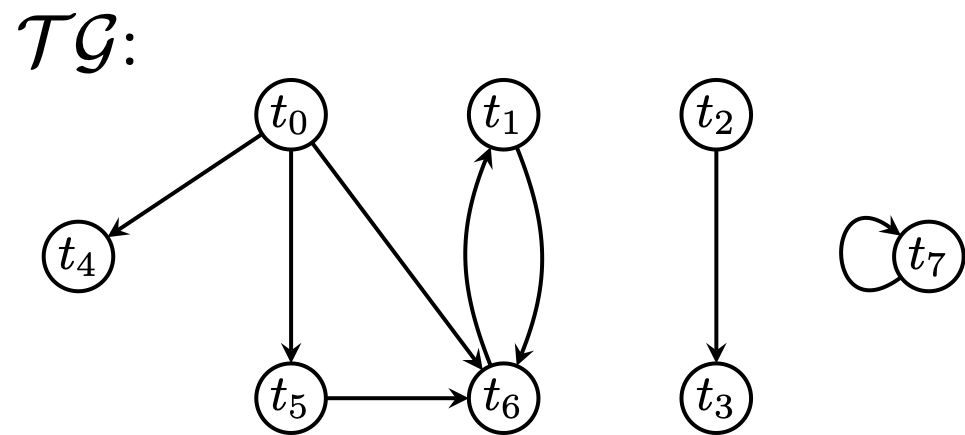
\includegraphics[width=0.75\columnwidth]{img/token-graph/token-graph.png}}
  \caption{A token graph, $\mathcal{TG}$, with eight vertices, $t_0,
    t_1, \ldots, t_7$, and eight edges.  Each edge corresponds to a
    token tokenising another token.  For example, the token
    represented by $t_5$ tokenises the token represented by
    $t_0$.}\label{fig:token-graph}
\end{figure}

We can construct a directed graph from the tokenising meta-events as
follows.  Each vertex corresponds to a token.  Each directed edge from
a source vertex to a target vertex corresponds to a set of tokenising
meta-events that deposits the source token and mints the target token,
and/or withdraws the source token and burns the target token.  In the
terminology of ERC~4626, the source token is the \textit{asset} and
the target token is the \textit{share}.  Figure~\ref{fig:token-graph}
shows an example token graph.

In the unfiltered case, the directed graph has \num{23687} vertices
(distinct tokens) and \num{23549} edges representing pairs of tokens
where the second tokenises the first with either deposit \& mint or
withdraw \& burn actions.  In the filtered case, the directed graph
has \num{8424} vertices that are incident with at least one edge and
\num{7536} edges representing pairs of tokens where the second
tokenises the first with both deposit \& mint and withdraw \& burn
actions.  We will refer to the \textit{unfiltered} and
\textit{filtered token graphs} in the remainder of the paper.

\subsection{Data Limitations}\label{sec:token-comp-limitations}

Our input data, namely, EVM logs, CoinGecko market data, and DEX
Screener liquidity pool data, have limitations.  Firstly, EVM logs are
unauthenticated: a contract can emit an event of its choosing.  There
is no guarantee that, say, an ERC-20 \texttt{Transfer} event
accurately reflects an actual transfer~\cite{guidi-michienzi-22}.
Furthermore, the first special case highlighted in
Sec.~\ref{sec:token-comp-evm-logs} (mint) is recommended by
ERC-20\footnote{``A token contract which creates new tokens SHOULD
trigger a Transfer event with the \texttt{\_from} address set to
\texttt{0x0} when tokens are
created.''~\cite{vogelsteller-buterin-15}} but the second (burn) is
not.  However, EVM logs for the Ethereum blockchain are generally
accurate and malicious contracts can be easily excluded.  For an
aggregated analysis, such as ours, we believe the impact of these
limitations are minimal.

Secondly, the data from CoinGecko and DEX Screener are snapshots that
were gathered in April 2024 whereas the EVM logs have a temporal
component.  It is possible that a token had an entry on CoinGecko in
the past, but, at the time the data was gathered, the entry no longer
existed.  It is also possible that a token was tracked by DEX Screener
in the past, but, at the time the data was gathered, it was no longer
being tracked.  It is also possible that the token coverage of
CoinGecko or DEX Screener is incomplete or inaccurate.  However, as a
high-level measure of token popularity, we believe the impact of this
potential mismatch is minimal.

Thirdly, tokenising meta-events are a heuristic for identifying
instances where one token is tokenised by another.  False positives
create edges in the token graph where the token corresponding to the
source is not tokenised by the token corresponding to the target;
false negatives are pairs of tokens where one is tokenised by the
other but there is no corresponding edge in the token graph.  We will
discuss both cases in Sec.~\ref{sec:analysis} and
Sec.~\ref{sec:conclusion}.


\section{Data}\label{sec:data}

\subsection{Ethereum Event Logs and Meta-Events}\label{sec:data-event-logs}

The Ethereum event logs record specific occurrences or outputs
generated during the execution of contract code.  They enable
off-chain applications to react to on-chain events.  A popular event
is the \texttt{Transfer} event emitted by ERC~20
tokens~\cite{vogelsteller-buterin-15}:

\begin{lstlisting}[language=Solidity,
    caption={The ERC~20 \texttt{Transfer} event specifies three
      parameters: \texttt{from}, \texttt{to}, and \texttt{value}.}]
  event Transfer(address indexed from,
                 address indexed to,
                 uint256 value);
\end{lstlisting}

The event has two special cases.  In the first, the \texttt{from}
address is the zero address (\texttt{0x0}) and the contract mints new
tokens.  In the second, the \texttt{to} address is the zero address
and the contract burns existing tokens.

A single transaction can emit multiple events.  We define a
\textit{meta-event} to be a sequence of events that match some pattern
and are emitted by a single transaction.  We define a
\textit{tokenising meta-event} to be a meta-event where the pattern is
two \texttt{Transfer} events: one must indicate a transfer of tokens
to the contract and another must indicate a new token being minted
(\textit{deposit \& mint}), or one must indicate a token being burned
and another must indicate a transfer of an existing token from the
contract (\textit{withdraw \& burn}.  Our aim is to identify instances
where a token is tokenised by another token.  In the terminology of
ERC~4626, a tokenising meta-event corresponds to either a
\texttt{Deposit} event or a \texttt{Withdraw} event.  However, our
tokenising meta-event does not require the contract to follow
ERC~4626.

\begin{table*}
  \centering
  \caption{Each tokenising meta-event contains the address of the
    source token, the address of the target token, one of two possible
    pairs of actions (deposit \& mint or withdraw \& burn), the amount
    of the source token that was deposited or withdrawn, the amount of
    the target token that was minted or burned, and a transaction
    hash.  The table includes four sample entries from the full set of
    \num{4032033} tokenising meta-events: the earliest and latest
    tokenising meta-events that have deposit \& mint and withdraw \&
    burn actions.}\label{tab:meta-events}
  \begin{tabular}{|c|c|c|r|r|c|}
    \hline
    Source Token &
    Target Token &
    Actions &
    Source Amount &
    Target Amount &
    Tx Hash\\
    \hline

    % 0x549a1226da1eadc6f1af7c41aef6adc638466ffd8630822637706632bf8666d3:
    % First deposit/mint.
    \texttt{ARC}~(\texttt{0xac709f}) &
    \texttt{SWT}~(\texttt{0xb12a3c}) & deposit \& mint & \textit{dust}
    & \textit{dust} & \texttt{0x549a12}\\

    % 0x2da2326c330cb1fa1330151b60453448e19b02981e45fb5dc2ed0980224ce625:
    % First withdraw/burn.
    \texttt{DGZ}~(\texttt{0x84178d}) &
    \texttt{preDGZ}~(\texttt{0x18aa6e}) & withdraw \& burn &
    \num{1371} & \num{150} & \texttt{0x2da232}\\

    % 0x5dbe32de3b682fc1c7dc181fbf74eabbb87583c4bdce371c2a997c54fca47bfb:
    % Last withdraw/burn.
    \texttt{BONE}~(\texttt{0x981303}) &
    \texttt{tBONE}~(\texttt{0xf7a038}) & withdraw \& burn & \num{5183}
    & \num{5160} & \texttt{0x5dbe32}\\

    % 0xb4281adc73ca60aef5c29e0ae7114d629c3769b7cf9fcf9e365f6cb140c8527a:
    % Last deposit/mint.
    \texttt{WETH}~(\texttt{0xc02aaa}) &
    \texttt{aWETH}~(\texttt{0x030ba8}) & deposit \& mint & \num{25} &
    \num{25} & \texttt{0xb4281a}\\

    \hline
  \end{tabular}
\end{table*}

We extracted all \texttt{Transfer} events from Ethereum mainnet from
block height \num{0} to \num{16685101} (February 2023) inclusive using
Geth's \texttt{eth\_getLogs} RPC method~\cite{geth-xx}.  From the
\texttt{Transfer} events, we identified \num{4032033} tokenising
meta-events using the pattern described above.
Table~\ref{tab:meta-events} shows a sample of the data.  The first
(resp., last) two rows are the earliest (resp., latest) two
occurrences of tokenising meta-events in the data that perform a
deposit \& mint, and a withdraw \& burn.

For example, the first row indicates a transaction that deposited a
dust amount of ARC~\cite{arcade-city-xx} to a contract in a one-to-one
exchange for newly minted SWT~\cite{swarm-city-xx} in January 2017.
The third row indicates a transaction that withdrew
\num{5183}~{BONE}~\cite{shiba-inu-xx} from a contract in exchange for
burning \num{5160}~\texttt{tBONE} in February 2023.  We are not
concerned with the individual utility or value of the tokens (or lack
thereof); we are only interested in the fact that Token~$\mathcal{X}$
can be deposited with a contract to mint Token~$\mathcal{Y}$, and/or
Token~$\mathcal{Y}$ can be burned by a contract to withdraw
Token~$\mathcal{X}$.

We filter the tokenising meta-events to include only those meta-events
that involve two tokens, Token~$\mathcal{X}$ and Token~$\mathcal{Y}$,
such that there is at least one instance of Token~$\mathcal{X}$ being
deposited with a contract to mint Token~$\mathcal{Y}$, and at least
one instance of Token~$\mathcal{Y}$ being burned by a contract to
withdraw Token~$\mathcal{X}$.  In other words, the ``and/or''
conjunction in the previous paragraph is replaced by ``and''.  This
excludes \textit{one-way token upgrades} where Token~$\mathcal{X}$ can
be deposited with a contract to mint Token~$\mathcal{Y}$ but
Token~$\mathcal{X}$ cannot be withdrawn from the contract, and
\textit{one-way token burns} where Token~$\mathcal{Y}$ can be burned
by a contract to withdraw Token~$\mathcal{X}$ but Token~$\mathcal{X}$
cannot be deposited with the contract to mint Token~$\mathcal{Y}$.  Of
the \num{4032033} tokenising meta-events, \num{3461723} meet the
additional criterion.  We will refer to the unfiltered and filtered
tokenising meta-events in Sect.~\ref{sec:data-token-graphs}.

\subsection{Off-Chain Data}\label{sec:data-off-chain}

CoinGecko~\cite{gecko-labs-xx} is a cryptocurrency data platform that
aggregates fundamental analysis of tokens including market price,
exchange volume, and market capitalisation.

DEX Screener~\cite{dex-screener-xx} stores, parses, and analyses
blockchain data to produce a token screener, charts, and analytics.
They cover many blockchains, decentralised exchanges, and tokens.

\subsection{The Token Graphs}\label{sec:data-token-graphs}

We can construct a directed graph from the tokenising meta-events as
follows.  Each vertex corresponds to a distinct token.  Each directed
edge from a source vertex to a target vertex corresponds to a set of
tokenising meta-events that deposits the source token and mints the
target token, and/or withdraws the source token and burns the target
token.  In the terminology of ERC~4626, the source token is the
\textit{asset} and the target token is the \textit{share}.

In the unfiltered case, the directed graph has \num{23687} vertices
(distinct tokens) and \num{23549} edges representing pairs of tokens
where the second tokenises the first with either deposit \& mint or
withdraw \& burn actions.  In the filtered case, the directed graph
has \num{8424} vertices that are incident with at least one edge and
\num{7536} edges representing pairs of tokens where the second
tokenises the first with both deposit \& mint and withdraw \& burn
actions.  We will refer to the unfiltered and filtered token graphs in
the remainder of the paper.

\subsection{Data Limitations}\label{sec:data-limitations}

Our input data, namely, Ethereum event logs, CoinGecko market data,
and DEX Screener liquidity pool data, have limitations.  Firstly,
Ethereum event logs are unauthenticated: a contract can emit an event
of its choosing.  There is no guarantee that, say, an ERC-20
\texttt{Transfer} event accurately reflects an actual
transfer~\cite{guidi-michienzi-22}.  Additionally, the first special
case highlighted in Sect.~\ref{sec:data-event-logs} is stipulated by
ERC-20\footnote{``A token contract which creates new tokens SHOULD
trigger a Transfer event with the \texttt{\_from} address set to
\texttt{0x0} when tokens are
created.''~\cite{vogelsteller-buterin-15}} but the second is not.
However, event logs are generally accurate and malicious contracts can
be easily excluded.  For an aggregated analysis, such as ours, the
impact should be minimal.

Secondly, the data from CoinGecko and DEX Screener are snapshots that
were gathered in April 2024 whereas the Ethereum event logs have a
temporal component.  It is possible that a token had an entry on
CoinGecko in the past, but, at the time the data was gathered, the
entry no longer existed.  It is also possible that a token was tracked
by DEX Screener in the past, but, at the time the data was gathered,
it was no longer being tracked.  It is also possible that CoinGecko's
and DEX Screener's coverage is incomplete or inaccurate.  However, as
a high-level measure of token popularity, the impact of the mismatch
should be minimal.

Thirdly, tokenising meta-events are a heurstic for identifying
instances where one token is tokenised by another.  False positives
create edges in the token graph where the token corresponding to the
source vertex is not tokenised by the token corresponding to the
target vertex; false negatives are pairs of tokens where one is
tokenised by the other but there is no corresponding edge in the token
graph.  We will discuss both cases in Sect.~\ref{sec:analysis} and
Sect.~\ref{sec:conclusion}.


\section{Analysis}\label{sec:analysis}

In this section we examine the macro-topological structure of the
unfiltered and filtered token graphs including degree distributions,
connected component structure, and cyclic structure.  We also examine
the micro-topological structure of some individual tokens.  We
visualise the composition of tokens and identify their direct and
transitive dependencies.

\begin{table}
  \centering
  \caption{Each edge in a token graph represents a set of tokenising
    meta-events.  The top five most significant edges in terms of the
    number of tokenising meta-events they contain are shown.  The
    results are the same for both the unfiltered and filtered token
    graphs, i.e., the same five edges are present in
    both.}\label{tab:most-significant-edges}
  \begin{tabular}{|c|c|r|}
    \hline

    Source Token & Target Token & \begin{tabular}{@{}c@{}}\#
      Tokenising\\Meta-Events\end{tabular}\\

    \hline

    \texttt{SHIB}~(\texttt{0x95ad61}) &
    \texttt{xSHIB}~(\texttt{0xb4a812}) & \num{402186}\\

    \texttt{BONE}~(\texttt{0x981303}) &
    \texttt{tBONE}~(\texttt{0xf7a038}) & \num{203734}\\

    \texttt{SUSHI}~(\texttt{0x6b3595}) &
    \texttt{xSUSHI}~(\texttt{0x879824}) & \num{120221}\\

    \texttt{LEASH}~(\texttt{0x27c70c}) &
    \texttt{xLEASH}~(\texttt{0xa57d31}) & \num{75180}\\

    \texttt{USDC}~(\texttt{0xa0b869}) &
    \texttt{aUSDC}~(\texttt{0xbcca60}) & \num{69373}\\

    \hline
  \end{tabular}
\end{table}

We note that each edge in a token graph represents a set of tokenising
meta-events.  Before examining the structure of the graphs, we can
identify the most significant edges in terms of the number of
tokenising meta-events they contain.
Table~\ref{tab:most-significant-edges} shows the results for both the
unfiltered and filtered token graphs.  Three of the five edges
represent the staking of memecoins
(\texttt{SHIB}~$\rightarrow$~\texttt{xSHIB},
\texttt{BONE}~$\rightarrow$~\texttt{tBONE}, and
\texttt{LEASH}~$\rightarrow$~\texttt{xLEASH}), one represents the
staking of a governance token for a decentralised exchange
(\texttt{SUSHI}~$\rightarrow$~\texttt{xSUSHI}), and one represents the
supply of a stablecoin to a decentralised lending market
(\texttt{USDC}~$\rightarrow$~\texttt{aUSDC}).  Of course, we could
also measure the significance of a edge based on, say, the volume of
tokens transacted, the present USD value of the locked tokens, etc.

\subsection{Degree Distributions}\label{sec:analysis-degree-distribution}

\begin{figure}
  \centerline{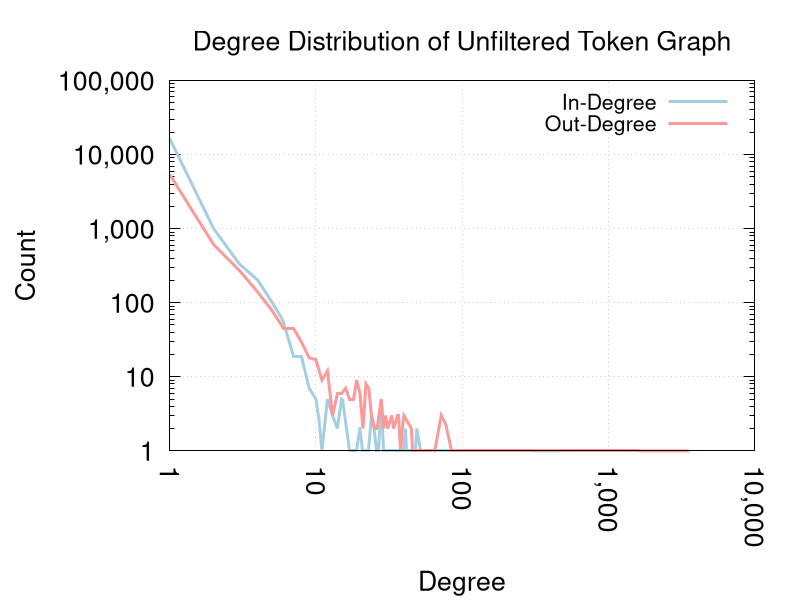
\includegraphics[width=\columnwidth]{img/degree-distributions/unfiltered-token-graph-degrees.png}}
  \caption{The in- and out-degree distributions of the unfiltered
    token graph show an inverse relationship between the degree of a
    vertex and the number of vertices with that degree in the graph.
    There are a small number of vertices with high degree and a large
    number of vertices with low
    degree.}\label{fig:unfiltered-token-graph-degrees}
\end{figure}

\begin{figure}
  \centerline{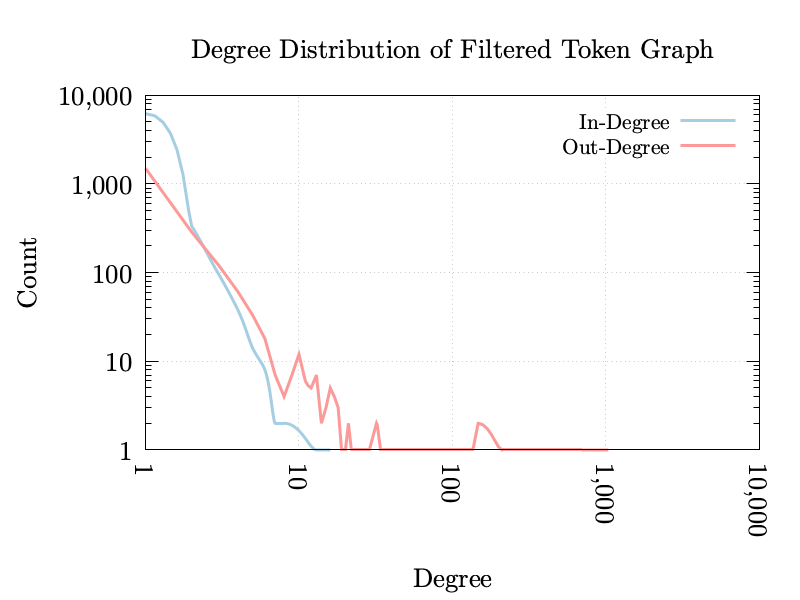
\includegraphics[width=\columnwidth]{img/degree-distributions/filtered-token-graph-degrees.png}}
  \caption{The in- and out-degree distributions of the filtered token
    graph show a similar inverse relationship as in
    Fig.~\ref{fig:unfiltered-token-graph-degrees}.}\label{fig:filtered-token-graph-degrees}
\end{figure}

\begin{table}
  \centering
  \caption{The top five vertices (tokens) in the unfiltered and
    filtered token graphs by in-degree and
    out-degree.}\label{tab:highest-in-out-degrees}
  \begin{tabular}{|c|c|r|c|r|}
    \hline

    & \multicolumn{2}{c|}{Top Five by In-Degree} &
    \multicolumn{2}{c|}{Top Five by Out-Degree}\\

    \cline{2-5}

    & Token & Deg. & Token & Deg.\\

    \hline

    \multirow{5}{0pt}{\rotatebox{90}{Unfiltered}}

    & \texttt{CHI}~(\texttt{0x000000}\footnote{The contract address
    for \texttt{CHI} is
    \texttt{0x0000000000004946c0e9f43f4dee607b0ef1fa1c}.}) & \num{471}
    & \texttt{USDC}~(\texttt{0xa0b869}) & \num{3587}\\

    & \texttt{USDP}~(\texttt{0x145668}) & \num{117} &
      \texttt{DAI}~(\texttt{0x6b1754}) & \num{1923}\\

    & \texttt{aUSDC}~(\texttt{0xbcca60}) & \num{84} &
      \texttt{USDT}~(\texttt{0xdac17f}) & \num{1175}\\

    & \texttt{aWETH}~(\texttt{0x030ba8}) & \num{63} &
      \texttt{WETH}~(\texttt{0xc02aaa}) & \num{951}\\

    & \texttt{aDAI}~(\texttt{0x028171}) & \num{54} &
      \texttt{sUSD}~(\texttt{0x57ab1e}) & \num{548}\\

    \hline

    \multirow{5}{0pt}{\rotatebox{90}{Filtered}}

    & \texttt{XDP2}~(\texttt{0xe68c1d}) & \num{16} &
    \texttt{USDC}~(\texttt{0xa0b869}) & \num{1037}\\

    & \texttt{XDP1}~(\texttt{0x134fc6}) & \num{15} &
    \texttt{DAI}~(\texttt{0x6b1754}) & \num{752}\\

    & \texttt{cyUSD}~(\texttt{0x1d0914}) & \num{14} &
    \texttt{USDT}~(\texttt{0xdac17f}) & \num{396}\\

    & \texttt{iDOL}~(\texttt{0x7591a3}) & \num{13} &
    \texttt{WETH}~(\texttt{0xc02aaa}) & \num{281}\\

    & \texttt{agEUR}~(\texttt{0x1a7e4e}) & \num{8} &
    \texttt{WBTC}~(\texttt{0x2260fa}) & \num{211}\\

    \hline
  \end{tabular}
\end{table}

The in- and out-degree distributions of the unfiltered and filtered
token graphs show an inverse relationship between the degree of a
vertex and the number of vertices with that degree in the graph (see
Fig.~\ref{fig:unfiltered-token-graph-degrees} and
Fig.~\ref{fig:filtered-token-graph-degrees}).
Table~\ref{tab:highest-in-out-degrees} shows the top five vertices in
the unfiltered and filtered token graphs by in-degree and out-degree.
The out-degree entries are easy to explain: they are the tokens that
are deposited with contracts in order to mint many other types of
tokens.  They include stablecoins (\texttt{USDC}, \texttt{DAI},
\texttt{USDT} and \texttt{sUSD}), wrapped ether (\texttt{WETH}), and
wrapped bitcoin (\texttt{WBTC}).  The in-degree entries are more
complex and have multiple explanations.  For example,
\texttt{CHI}~\cite{1inch-20} is a gas token created by 1inch, a
decentralised exchange aggregator, that is burned to obtain a
reduction in transaction fees; in some transactions the burning of
\texttt{CHI} is combined with the withdrawal of another token.  This
is a false positive generated by our heuristic since \texttt{CHI} does
not tokenise a token.  The remaining in-degree entries in the
unfiltered category are due to token swaps performed during a deposit.
For example, \texttt{aDAI}~\cite{aave-xx} is a yield-bearing token
issued by AAVE, a decentralised lending market, in exchange for the
stablecoin \texttt{DAI}.  However, in some transactions, other tokens
are supplied and swapped to \texttt{DAI}.  These are also false
positives since only \texttt{DAI} is tokenised by \texttt{aDAI}.  In
the filtered category, the in-degree entries are more reliable.  For
example, the \texttt{iDOL} token is minted when a user deposits
various forms of the \texttt{SBT} token (e.g., \texttt{SBT09180200},
\texttt{SBT09250200}, etc.) according to the Lien
Protocol~\cite{lien-20}.  Similarly, the \texttt{agEUR} token is a
stablecoin by the Angle Protocol~\cite{angle-xx} that accepts a
variety of tokens as collateral.

\begin{figure}
  \centerline{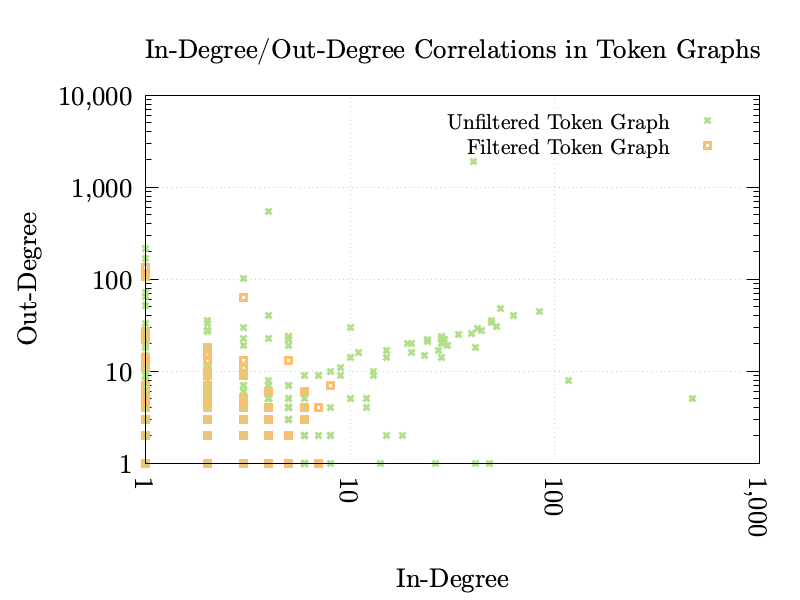
\includegraphics[width=\columnwidth]{img/degree-distributions/token-graph-in-out-degrees.png}}
  \caption{In the unfiltered and filtered token graphs, we can
    identify vertices with both high in-degree and high
    out-degree.}\label{fig:token-graph-in-out-degrees}
\end{figure}

Figure~\ref{fig:token-graph-in-out-degrees} plots in-degrees against
out-degrees in the unfiltered and filtered token graphs.  The tokens
whose corresponding vertices have both high in-degree and high
out-degree are tokens that tokenise many other tokens, and are
themselves tokenised by many other tokens.  Examples include
\texttt{mUSD}, a stablecoin issued by the mStable
protocol~\cite{mstable-xx} and the \texttt{agEUR} token.  This makes
intuitive sense as stablecoins can be minted from various forms of
collateral, and stablecoins can be used as collateral to mint other
tokens.

\subsection{Connected Component Structure}\label{sec:analysis-component-structure}

The unfiltered graph has \num{4082} weakly connected components.  A
giant component contains \num{13794} vertices ($\sim$\num{58}\%) and
\num{17711} edges ($\sim$\num{75}\%).  \num{3336} components
($\sim$\num{82}\% of the total) contain two connected vertices.  These
vertices correspond to pairs of tokens where at least one tokenises
the other, but neither tokenises, or is tokenised by, a third.
Interestingly, none of the tokens represented by vertices in these
components have a non-zero market capitalisation according to
CoinGecko or are traded in a liquidity pool according to DEX Screener.
Their lack of popularity reflects their isolation in the token graph.

\begin{figure}
  \centerline{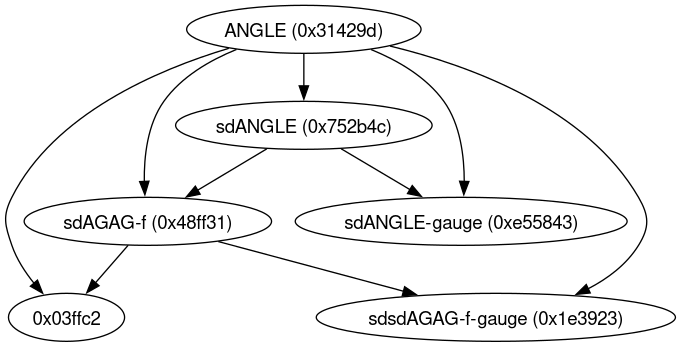
\includegraphics[width=\columnwidth]{img/medium-components/angle-protocol.png}}
  \caption{The unfiltered token graph contains a weakly connected
    component whose vertices correspond to tokens related to the Angle
    Protocol and Stake DAO.}\label{fig:angle-protocol}
\end{figure}

There are \num{418} components, other than the giant component, with
more than two connected vertices.  Figure~\ref{fig:angle-protocol} is
an example from this set.  It shows the tokenising relationships
between tokens related to the Angle Protocol~\cite{angle-xx} and Stake
DAO~\cite{stake-dao-xx}.  Stake DAO implements investment strategies
based on other decentralised protocols.  Their ``Liquid Lockers''
produce liquidity, voting power, and yield from lockable tokens.
\texttt{ANGLE} is Angle's governance token.  It can be deposited with
Stake DAO to mint \texttt{sdANGLE}.  It is not possible to burn
\texttt{sdANGLE} and withdraw \texttt{ANGLE}: the edge between those
vertices represents a one-way operation and is present in the
unfiltered token graph but not in the filtered version. \texttt{ANGLE}
and \texttt{sdANGLE} can be deposited in a gauge (liquidity pool) to
mint \texttt{sdANGLE-gauge}.  We can use this visualisation to
identify the direct and transitive dependencies of tokenising tokens
such as \texttt{sdANGLE} and \texttt{sdANGLE-gauge}.  Many of the
other components in the set produce similar insights that relate to
other tokens and protocols.

\begin{figure*}
  \centerline{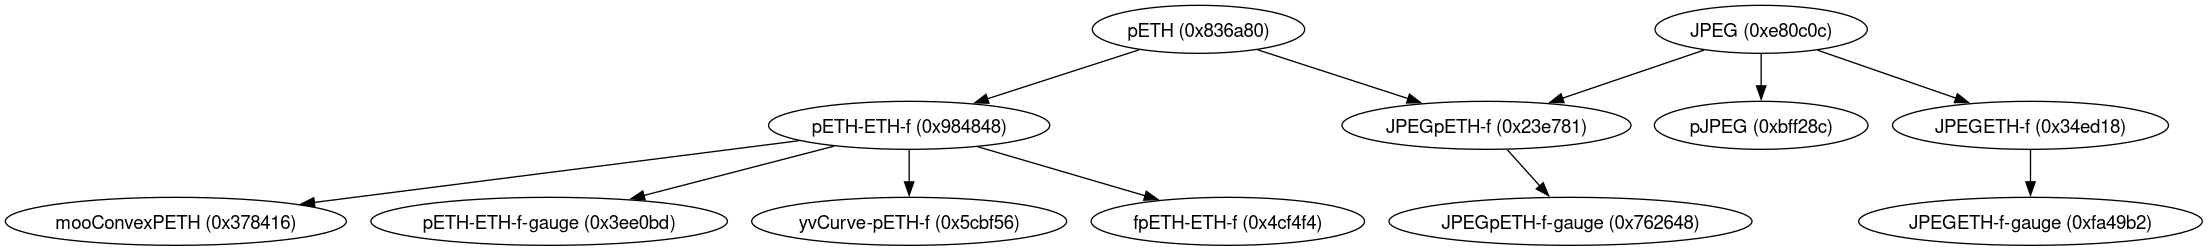
\includegraphics[width=\textwidth]{img/medium-components/jpegd-protocol.png}}
  \caption{The filtered token graph contains a weakly connected
    component whose vertices correspond to tokens related to the
    JPEG'd Protocol.}\label{fig:jpegd-protocol}
\end{figure*}

The filtered graph has \num{1491} weakly connected components.  A
giant component contains \num{4648} vertices ($\sim$\num{55}\%) and
\num{5247} edges ($\sim$\num{70}\%).  \num{1162} components
($\sim$\num{78}\% of the total) contain two connected vertices.  There
are \num{196} components, other than the giant component, with more
than two connected vertices.  Figure~\ref{fig:jpegd-protocol} is an
example from this set that relates to the JPEG'd
Protocol~\cite{jpegd-xx}.  JPEG'd is a decentralised lending market
where users can supply non-fungible-tokens (NFTs) as collateral and
obtain loans in \texttt{pETH}, a synthetic token that tracks the price
of ether. \texttt{JPEG} is the protocol's governance token.  The
figure shows the various ways in which \texttt{pETH} and \texttt{JPEG}
can be tokenised by liquidity pools such as Curve's \texttt{pETH/WETH}
pool~\cite{curve-finance-xx}. Unlike the operations represented by
edges in Fig.~\ref{fig:angle-protocol}, all operations represented by
edges in Fig.~\ref{fig:jpegd-protocol} can be reversed by burning the
tokenising tokens and withdrawing the underlying.

Both the unfiltered and filtered graphs contain giant weakly connected
components.  Exploring such structures requires an interactive user
interface with navigational aids such as selection, panning, and
zooming.  As an illustrative example of the interesting structure in
the giant components, we identified the longest directed path in the
filtered token graph.  It comprises nine vertices and represents the
following sequence of tokens:

\begin{enumerate}
\item \texttt{renBTC}~(\texttt{0xeb4c27})
\item \texttt{sBTC}~(\texttt{0xfe18be})
\item \texttt{crvRenWSBTC}~(\texttt{0x075b1b})
\item \texttt{tbtc/sbtcCrv}~(\texttt{0x64eda5})
\item \texttt{btbtc/sbtcCrv}~(\texttt{0xb9d076})
\item \texttt{ibBTC}~(\texttt{0xc4e159})
\item \texttt{wibBTC}~(\texttt{0x8751d4})
\item \texttt{ibbtc/sbtcCRV-f}~(\texttt{0xfbdca6})
\item \texttt{bibbtc/sbtcCRV-f}~(\texttt{0xae96ff})
\end{enumerate}

\texttt{renBTC} can be deposited with a contract to mint
\texttt{sBTC}, \texttt{sBTC} can be deposited with a contract to mint
\texttt{crvRenWSBTC}, etc.  The reverse operations can also be
performed (withdraw \& burn).  The chain involves tokens from several
different protocols.  It is an example of ``composition in the wild''
--- groups of interacting smart contracts than span multiple
protocols.

\subsection{Cyclic Structure}\label{sec:analysis-cyclic-structure}


\section{Conclusion}\label{sec:conclusion}

In many fields, including engineering, chemistry, and cooking, the
complexity of a product arises from the combination of numerous base
materials or ingredients.  This principle holds true for tokens on
blockchains.  For example,
\texttt{stkcvxcrvRenWBTC-abra}~(\texttt{0xb65ede}) is a token that
represents a staked deposit of a share of a liquidity pool for
synthetic and wrapped versions of Bitcoin's native token.  The base
tokens (\texttt{renBTC}~(\texttt{0xeb4c27}),
\texttt{wBTC}~(\texttt{0x2260fa}), etc.) are combined to produce the
product.  In this paper we detail a novel graph representation of
token composition.  We construct the graph from the EVM logs of the
Ethereum blockchain and we relate its properties to the tokenisation
process.  For example, we highlight the role of stablecoins that can
be minted from various forms of collateral, and can be used as
collateral to mint other tokens.  In future work, we will refine the
heuristic for identifying tokenising meta-events to reduce the number
of false positives in the token graph.


\bibliographystyle{IEEEtran}
\bibliography{bib/main}

\end{document}
